\documentclass[14pt]{extbook}
\usepackage{multicol, enumerate, enumitem, hyperref, color, soul, setspace, parskip, fancyhdr} %General Packages
\usepackage{amssymb, amsthm, amsmath, bbm, latexsym, units, mathtools} %Math Packages
\everymath{\displaystyle} %All math in Display Style
% Packages with additional options
\usepackage[headsep=0.5cm,headheight=12pt, left=1 in,right= 1 in,top= 1 in,bottom= 1 in]{geometry}
\usepackage[usenames,dvipsnames]{xcolor}
\usepackage{dashrule}  % Package to use the command below to create lines between items
\newcommand{\litem}[1]{\item#1\hspace*{-1cm}\rule{\textwidth}{0.4pt}}
\pagestyle{fancy}
\lhead{Makeup Progress Quiz -1}
\chead{}
\rhead{Version A}
\lfoot{7547-2949}
\cfoot{}
\rfoot{Fall 2020}
\begin{document}

\begin{enumerate}
\litem{
Choose the graph of the equation below.\[ f(x) = - \sqrt{x - 14} + 5 \]\begin{enumerate}[label=\Alph*.]
\begin{multicols}{2}\item 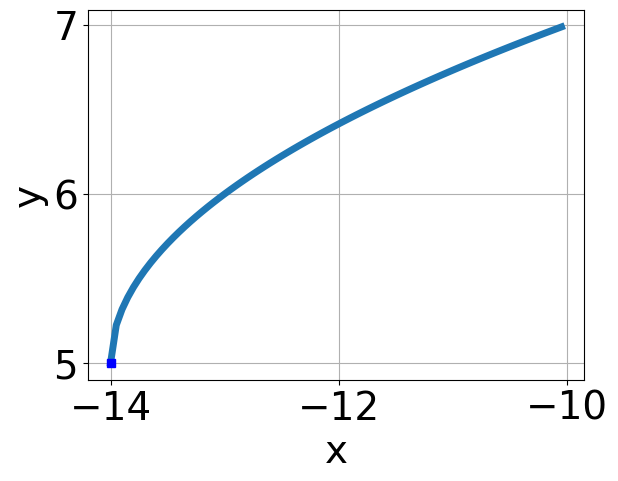
\includegraphics[width = 0.3\textwidth]{../Figures/radicalEquationToGraphCopyAA.png}\item 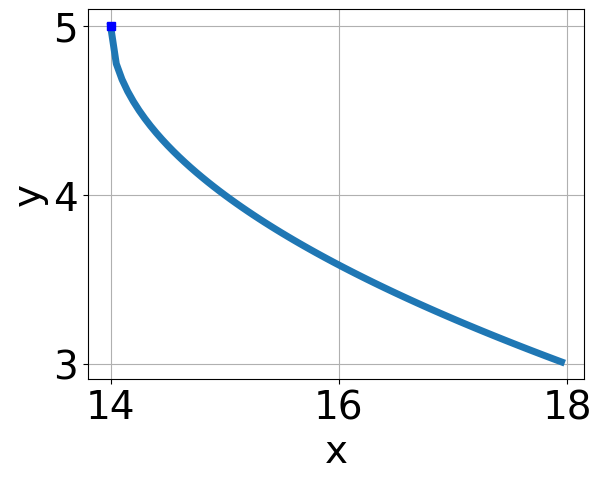
\includegraphics[width = 0.3\textwidth]{../Figures/radicalEquationToGraphCopyBA.png}\item 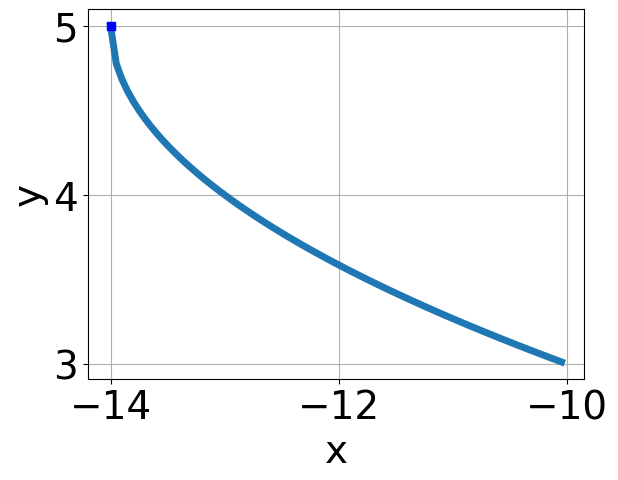
\includegraphics[width = 0.3\textwidth]{../Figures/radicalEquationToGraphCopyCA.png}\item 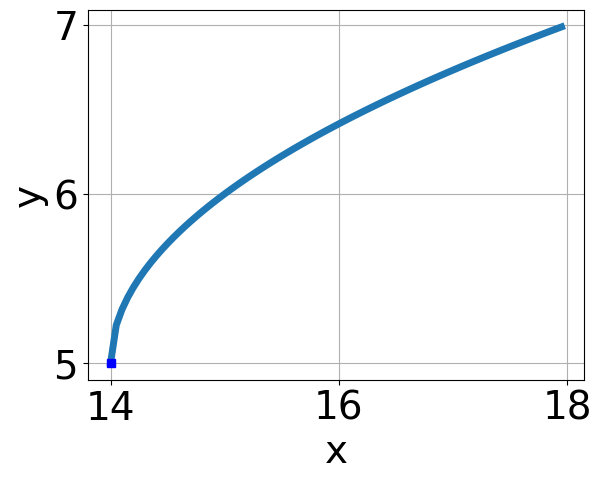
\includegraphics[width = 0.3\textwidth]{../Figures/radicalEquationToGraphCopyDA.png}\end{multicols}\item None of the above.
\end{enumerate} }
\litem{
Choose the graph of the equation below.\[ f(x) = \sqrt[3]{x - 8} + 5 \]\begin{enumerate}[label=\Alph*.]
\begin{multicols}{2}\item 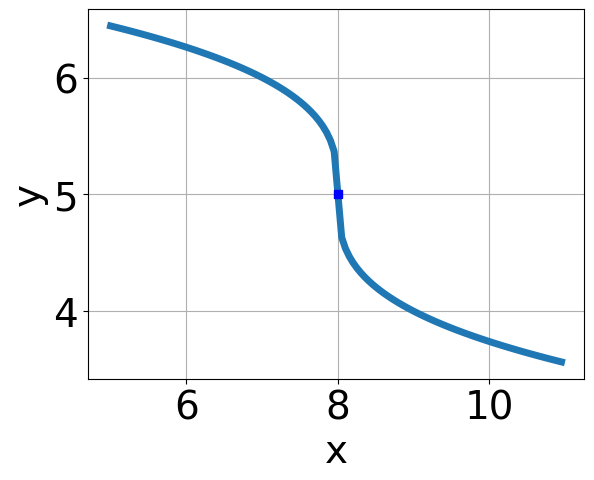
\includegraphics[width = 0.3\textwidth]{../Figures/radicalEquationToGraphAA.png}\item 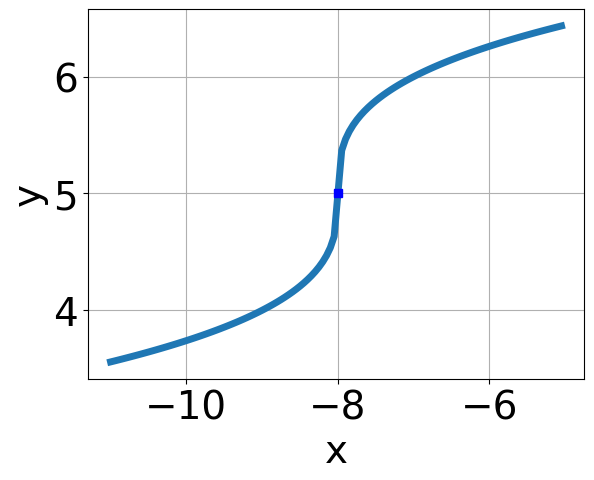
\includegraphics[width = 0.3\textwidth]{../Figures/radicalEquationToGraphBA.png}\item 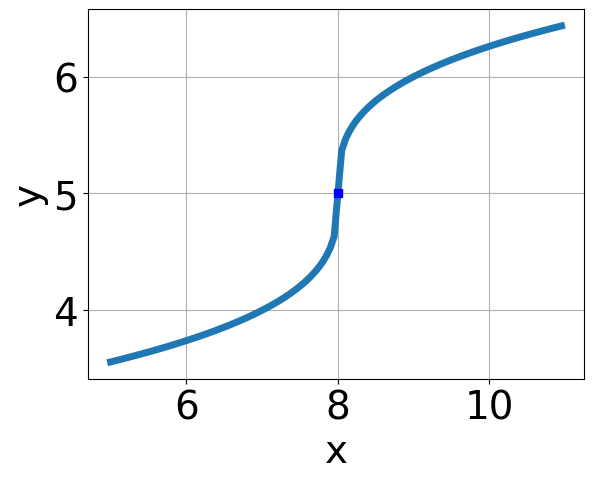
\includegraphics[width = 0.3\textwidth]{../Figures/radicalEquationToGraphCA.png}\item 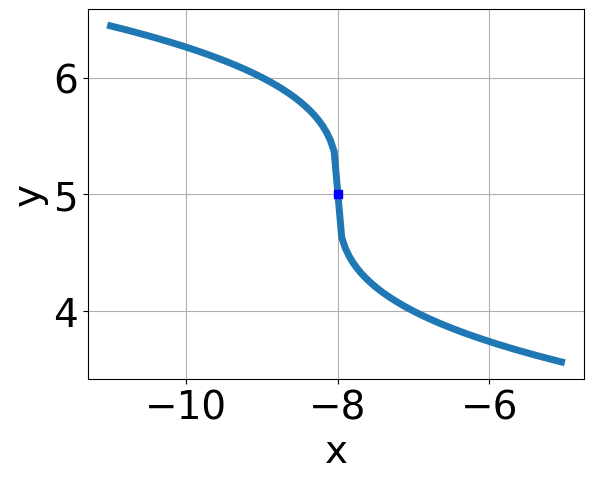
\includegraphics[width = 0.3\textwidth]{../Figures/radicalEquationToGraphDA.png}\end{multicols}\item None of the above.
\end{enumerate} }
\litem{
Solve the radical equation below. Then, choose the interval(s) that the solution(s) belongs to.\[ \sqrt{-20 x^2 + 30} - \sqrt{10 x} = 0 \]\begin{enumerate}[label=\Alph*.]
\item \( x_1 \in [-5.5, 0.5] \text{ and } x_2 \in [0.85,1.37] \)
\item \( \text{All solutions lead to invalid or complex values in the equation.} \)
\item \( x \in [-5.5,0.5] \)
\item \( x \in [0,8] \)
\item \( x_1 \in [0, 8] \text{ and } x_2 \in [1.4,1.62] \)

\end{enumerate} }
\litem{
Solve the radical equation below. Then, choose the interval(s) that the solution(s) belongs to.\[ \sqrt{2 x - 9} - \sqrt{5 x - 8} = 0 \]\begin{enumerate}[label=\Alph*.]
\item \( \text{All solutions lead to invalid or complex values in the equation.} \)
\item \( x_1 \in [0.3, 2.6] \text{ and } x_2 \in [2.5,10.5] \)
\item \( x \in [-0.8,1] \)
\item \( x \in [-7.7,-4.9] \)
\item \( x_1 \in [-0.8, 1] \text{ and } x_2 \in [2.5,10.5] \)

\end{enumerate} }
\litem{
Choose the equation of the function graphed below.
\begin{center}
    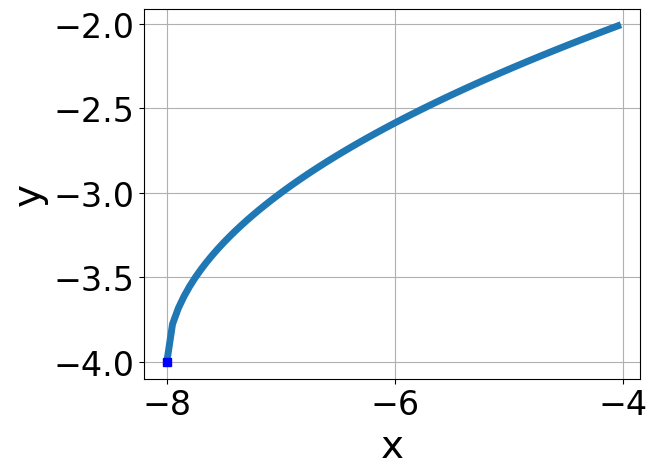
\includegraphics[width=0.5\textwidth]{../Figures/radicalGraphToEquationA.png}
\end{center}
\begin{enumerate}[label=\Alph*.]
\item \( f(x) = \sqrt[3]{x + 8} - 4 \)
\item \( f(x) = - \sqrt[3]{x + 8} - 4 \)
\item \( f(x) = - \sqrt[3]{x - 8} - 4 \)
\item \( f(x) = \sqrt[3]{x - 8} - 4 \)
\item \( \text{None of the above} \)

\end{enumerate} }
\litem{
What is the domain of the function below?\[ f(x) = \sqrt[5]{6 x + 8} \]\begin{enumerate}[label=\Alph*.]
\item \( \text{The domain is } (-\infty, a], \text{   where } a \in [-1.17, 0.24] \)
\item \( (-\infty, \infty) \)
\item \( \text{The domain is } [a, \infty), \text{   where } a \in [-0.97, 1.14] \)
\item \( \text{The domain is } [a, \infty), \text{   where } a \in [-2.01, -0.9] \)
\item \( \text{The domain is } (-\infty, a], \text{   where } a \in [-3.24, -1.16] \)

\end{enumerate} }
\litem{
Choose the equation of the function graphed below.
\begin{center}
    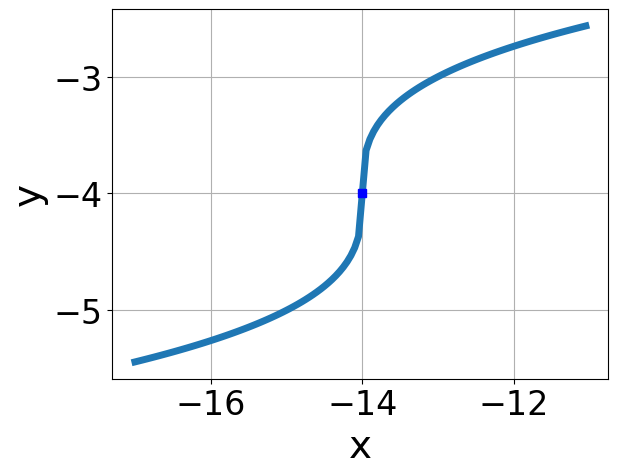
\includegraphics[width=0.5\textwidth]{../Figures/radicalGraphToEquationCopyA.png}
\end{center}
\begin{enumerate}[label=\Alph*.]
\item \( f(x) = \sqrt[3]{x + 14} - 4 \)
\item \( f(x) = \sqrt[3]{x - 14} - 4 \)
\item \( f(x) = - \sqrt[3]{x + 14} - 4 \)
\item \( f(x) = - \sqrt[3]{x - 14} - 4 \)
\item \( \text{None of the above} \)

\end{enumerate} }
\litem{
What is the domain of the function below?\[ f(x) = \sqrt[3]{9 x + 8} \]\begin{enumerate}[label=\Alph*.]
\item \( \text{The domain is } [a, \infty), \text{   where } a \in [-1.55, -1.07] \)
\item \( \text{The domain is } (-\infty, a], \text{   where } a \in [-0.9, -0.87] \)
\item \( \text{The domain is } [a, \infty), \text{   where } a \in [-0.97, 0.11] \)
\item \( \text{The domain is } (-\infty, a], \text{   where } a \in [-1.16, -0.98] \)
\item \( (-\infty, \infty) \)

\end{enumerate} }
\litem{
Solve the radical equation below. Then, choose the interval(s) that the solution(s) belongs to.\[ \sqrt{-45 x^2 - 48} - \sqrt{94 x} = 0 \]\begin{enumerate}[label=\Alph*.]
\item \( x \in [-0.91,-0.77] \)
\item \( x_1 \in [-1.33, -1.16] \text{ and } x_2 \in [-2.89,0.11] \)
\item \( x_1 \in [0.54, 1.44] \text{ and } x_2 \in [-0.11,6.89] \)
\item \( x \in [-1.33,-1.16] \)
\item \( \text{All solutions lead to invalid or complex values in the equation.} \)

\end{enumerate} }
\litem{
Solve the radical equation below. Then, choose the interval(s) that the solution(s) belongs to.\[ \sqrt{3 x - 4} - \sqrt{4 x - 4} = 0 \]\begin{enumerate}[label=\Alph*.]
\item \( x \in [-0.22,0.61] \)
\item \( x \in [-8.71,-6.71] \)
\item \( x_1 \in [0.82, 1.31] \text{ and } x_2 \in [-1.67,3.33] \)
\item \( x_1 \in [-0.22, 0.61] \text{ and } x_2 \in [-1.67,3.33] \)
\item \( \text{All solutions lead to invalid or complex values in the equation.} \)

\end{enumerate} }
\end{enumerate}

\end{document}